
\chapter{Generalized Adaptive Intelligent Binning of Multiway Data}

\begin{quote}
{\it
  The art of doing mathematics consists in finding that special case which
  contains all the germs of generality.}
\\\\
 -- David Hilbert
\end{quote}

\section{Introduction}

\begin{figure}[hb!]
\includegraphics[width=6in]{figs/gaibin/01-scheme.png}
\caption
      [Generalization of Adaptive Intelligent Binning.]{
  {\bf Generalization of Adaptive Intelligent Binning.}
  \\
  ({\bf A}) In the one-dimensional case, the bin containing regions 1 and 2
  is optimally subdivided ({\it asterisk}) when the sum of the objective values
  in regions 1 and 2 is maximal and greater than the original bin's objective
  value. ({\bf B}) In the $D$-dimensional case, there are now $D$ possible
  dimensions along which an optimal subdivision may exist. The optimal
  subdivision along the \hnmr{} dimension ({\it triangle}) occurs when the sum
  of the objective values in regions 3+6 and 4+5 is maximal and greater than
  that of the original bin. Similarly, the optimal subdivision along the
  \cnmr{} dimension ({\it circle}) occurs when the sum of the objective values
  in regions 3+4 and 5+6 is maximal and above the original bin objective. A
  comparison between all possible optimal subdivisions along all dimensions
  yields the best possible subdivision (\cnmr{}, {\it circle}).
}
\label{figure.8.1}
\end{figure}

\begin{doublespace}
By and large, the phase ``NMR metabolic fingerprinting'' implies the use of
one-dimensional (1D) \hnmr{} NMR spectroscopic methods, due in no small part
to the ease and speed of 1D data collection and the large natural abundance
of NMR-active protons found in metabolomics samples
\cite{lindon:cmr2000,worley:cmb2013}. Before processed spectra are
submitted to PCA or PLS for modeling, they are often subdivided into bins
to simplify multivariate analyses. Spectral binning, introduced and described
in detail in \hyperlink{chapter.3}{Chapter 3}, reduces the dimensionality of
a data matrix and masks chemical shift variability between samples at the
expense of decreased model interpretability: any given bin in a 1D \hnmr{} NMR
spectral dataset may contain several overlapped signals from multiple distinct
metabolites \cite{aberg:abc2009}. Thus, without utilizing
computationally intensive methods of deconvolution to tease apart signal
contributions from individual metabolites
\cite{astle:jasa2012,zheng:binf2011}, the resulting fingerprint from a
binned 1D dataset is usually limited to high-level inference about metabolic
trends.
\\\\
By leveraging the connectivities between \hnmr{} and \cnmr{} nuclei in
metabolites, two-dimensional (2D) heteronuclear NMR methods reduce spectral
overlap by spreading \hnmr{} information over a second (\cnmr) chemical shift
dimension \cite{mandal:cmr2004}. Heteronuclear single quantum coherence (HSQC)
experiments are commonly performed in NMR metabolic profiling studies, and
provide an NMR singlet or multiplet for each directly bonded \hcnmr{} pair
in the sample. Developments in NMR hardware and acquisition techniques have
brought natural abundance \hcnmr{} HSQC experiment times down to values
compatible with high-throughput metabolic fingerprinting studies
\cite{motta:anchem2010,rai:anchem2012}. However, multivariate analysis
of 2D NMR datasets is still a nontrivial undertaking that requires either
vectorization \cite{hedenstrom:cils2008}, which breaks the inherent
structure of the data, or the use of multilinear factorizations
\cite{lu:ieee2009,lu:pr2011}, which are more computationally intensive
and difficult to cross-validate.
\\\\
Spectral binning is another potential means of preparing 2D NMR datasets for
multivariate analysis that holds several advantages over binning 1D spectra.
First, multiple integration of bins maps each spectrum to an observation
vector regardless of its original dimensionality, allowing bilinear PCA and
PLS algorithms to be used without concern for loss of the inherent structure
of the data. Second, binning of 2D spectral data yields more well-conditioned
data matrices than simple vectorization. Finally, because signals are better
resolved in 2D spectra, each bin contains substantially fewer signals from
distinct metabolites. Multiple different algorithms have been developed to
bin 1D NMR data \cite{
  anderson:metab2008,
  anderson:metab2011,
  davis:cils2007,
  demeyer:anchem2008,
  sousa:cils2013}, and the use of uniform binning on 2D NMR data has also been
reported \cite{van:jpr2008}. However, at the time of this writing, no methods
exist to \emph{intelligently} bin multidimensional data for use in multivariate
analyses. This motivated the development of a generalization of Adaptive
Intelligent (AI) binning \cite{demeyer:anchem2008} to spectral data
of any dimensionality, called Generalized Adaptive Intelligent (GAI) binning
(\figref{8.1}{Figure 8.1}).
\end{doublespace}

\section{Theory}

\subsection{AI-binning}

\begin{doublespace}
Generalized AI-binning (GAI-binning) is a logical extension of AI-binning to
two or more dimensions. In the AI algorithm (\figref{8.1}{Figure 8.1A}), bins
are recursively subdivided until a stopping criterion or minimum bin width is
reached \cite{demeyer:anchem2008}. For a 1D dataset containing $N$ spectra,
the following objective function is used to assess the quality of each bin:
\begin{equation}
V_b = \frac{1}{N}
  \sum_{n=1}^N \left[
    (max_{n,b} - I_{n,b,1})
    (max_{n,b} - I_{n,b,end}) \right]^\frac{R}{2}
\end{equation}
where $max_{n,b}$ is the maximum intensity inside the bin $b$ in spectrum $n$,
and $I_{n,b,1}$ and $I_{n,b,end}$ are the bin edge intensities. The exponent
$R$ in the AI objective function is referred to as a ``resolution parameter'',
which offers a means of tuning the binning result based on signal-to-noise and
peak resolution of a dataset. The replacement of $R$ with $\frac{R}{2}$ in the
exponent of equation 6.1, enables a slightly modified interpretation of each
summed term in the AI objective function as a relaxed form of a geometric mean
of the differences between the bin edge intensities and the maximum bin
intensity. At each subdivision step, new bin edges are chosen to maximize the
combined (summed) objective values of the two resulting bins over the objective
value of the original bin. If no bin subdivision exists with a combined
objective value greater than that of the original bin, recursive subdivision
within that bin is terminated, and the AI algorithm terminates once all bins
may no longer be subdivided.
\end{doublespace}

\subsection{GAI-binning}

\begin{doublespace}
In two or more dimensions, the set of bin boundary points expands to include
all points that lie on the edges (or faces, hyperfaces, etc.) of the bin.
By denoting the set of all edge points in bin $b$ as $E_b$, a new objective
function may be constructed:
\begin{equation}
V_b = \frac{1}{N}
  \sum_{n=1}^N \left[
    \prod_{e \in E_b} (max_{n,b} - I_e)
  \right]^\frac{R}{||E_b||}
\end{equation}

Thus, the GAI algorithm computes the ``relaxed'' geometric mean of the
differences between the bin maximum and all points on the boundary. In the
case of one-dimensional data, it is apparent that equation 6.2 reduces to
equation 6.1, and GAI-binning operates identically to AI-binning. As
dimensionality increases, the risk of floating-point overflow or underflow
increases due to the larger bin edge set $E_b$. To avoid this, the following
``log-objective'' may be used in lieu of equation 6.2:
\begin{equation}
V_{b,ln} = \frac{R}{N ||E_b||}
  \sum_{n=1}^N \sum_{e \in E_b}
    \ln(max_{n,b} - I_e)
\end{equation}

Like AI-binning, GAI-binning initializes a bin around the entire dataset and
proceeds to recursively subdivide each bin until a minimum bin size is reached
or no bin may be divided to yield an increase in the objective value. Because
the number of ways to subdivide each bin increases with dimensionality, all
possible dimensions are tested, and the new bin boundary that maximizes the
objective over all possible subdivision dimensions is selected
(\figref{8.1}{Figure 8.1B}). Therefore, the GAI algorithm may be considered
a form of binary space partitioning (BSP) which limits its partition
hyperplanes to lying orthogonally to the basis vectors of the coordinate
system \cite{deberg2000}.
\end{doublespace}

\subsection{Noise Bin Elimination}

\begin{doublespace}
It is important that noise bins be removed from the data matrix prior to
multivariate analysis, as their presence is known to negatively impact the
interpretability and reliability of multivariate models
\cite{halouska:jmr2006,bro:anmeth2014}. Because the integration of a
noisy space of increasing dimensionality (i.e. double or triple
integration) results in a random variable having a similarly increasing
variance, the importance of noise removal is compounded in multidimensional
binning. Therefore, a noise bin removal step based on spectral intensity was
added to the GAI algorithm. A running mean and variance calculation was
performed to estimate the noise floor of each spectrum. The initial mean
$\mu_n$ and standard deviation $\sigma_n$ of the noise were computed using the
first 32 points on one edge of the spectrum, which were assumed to contain only
baseline noise. Every other data point was then classified as signal or noise
based on whether its intensity exceeded the current running noise floor,
$\mu_n + 3 \sigma_n$. Upon inclusion of a new noise data point, the mean and
standard deviation of the noise were appropriately updated. Once the estimated
noise floor was determined for each spectrum in the dataset, a threshold for
bin removal was computed as the median noise floor of all the spectra:
\begin{equation}
I_{th} = \mathrm{med}_n (\mu_n + k \sigma_n)
\end{equation}
where $k$ is a user-selectable parameter to adjust the noise threshold. Only
bins whose maximum intensity fell above $I_{th}$ were retained in the final
data matrix.
\end{doublespace}

\section{Materials and Methods}

\subsection{Human Liver Dataset}

\begin{doublespace}
Two independently collected \hcnmr{} HSQC NMR datasets from ongoing
metabolomics studies were used as test cases for the GAI-binning algorithm.
For the first dataset, twenty-four 1.0 mL samples of SK-Hep1 human liver cells
were provided for metabolic fingerprinting, half of which were treated with
50 $\mu$M tetrathiomolybdate (TTM). The cells were extracted into 80:20
methanol:water to collect the water-soluble metabolites, spun in a rotary
evaporator for two hours, lyophilized at $-50^\circ$C and 0.02 mBar for 24
hours, and finally redissolved in 600 $\mu$L of 50.0 mM phosphate buffer in
99.8\% D$_2$O (Isotec, St. Louis, MO) adjusted to pH 7.4. The redissolved,
pH-adjusted samples were then collected into NMR tubes.
\\\\
Experiments were collected on a Bruker Avance III HD 700 MHz spectrometer
equipped with a 5 mm inverse quadruple-resonance (\hnmr{}, \cnmr{}, \nnmr{},
\pnmr{}) cryoprobe with cooled \hnmr{} and \cnmr{} channels and a {\it z}-axis
gradient. A Bruker SampleJet and ICON-NMR were used to automate NMR data
collection. A 2D gradient-enhanced \hcnmr{} HSQC with improved sensitivity
\cite{palmer:jmr1991,kay:jacs1992} ({\it hsqcetgpsi}) was collected for
each sample. Spectra were collected with 4 scans and 16 dummy scans over a
uniform Nyquist grid of 512 and 64 complex points along the \hnmr{} and \cnmr{}
dimensions, respectively. Spectral windows were set to 3,285 $\pm$ 4,545 Hz
along \hnmr{} and 12,677 $\pm$ 14,620 Hz along \cnmr{}. All spectra were
collected at a sample temperature of 298.0 K.
\end{doublespace}

\begin{figure}[hb!]
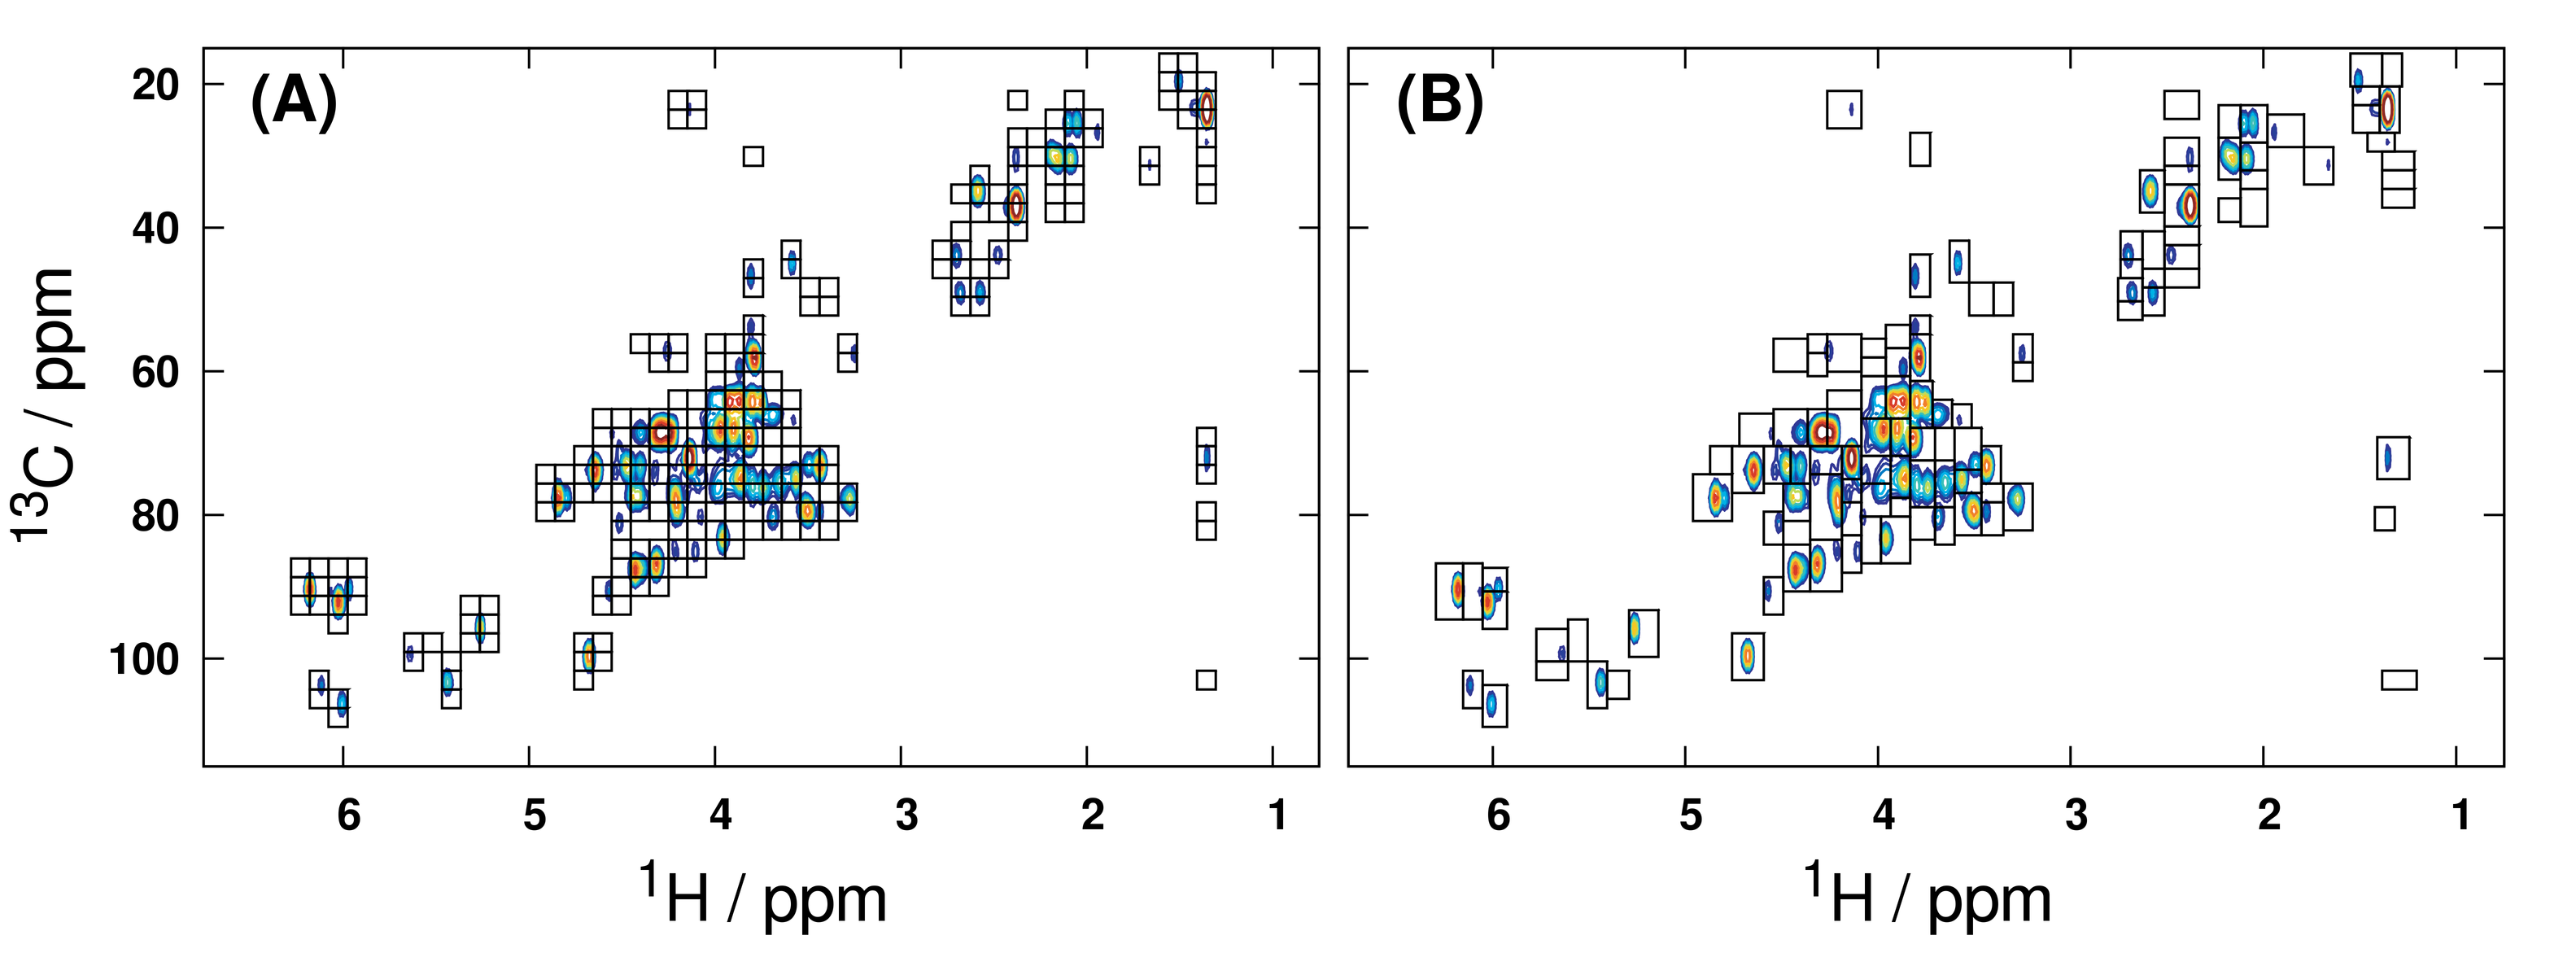
\includegraphics[width=6in]{figs/gaibin/02-hsqc-liver.png}
\caption
      [Binned Liver Dataset.]{
  {\bf Binned Liver Dataset.}
  \\
  Processed \hcnmr{} HSQC mean spectrum of the liver data tensor, with
  overlaid uniform ({\bf A}) and GAI ({\bf B}) bin boundaries.
}
\label{figure.8.2}
\end{figure}

\subsection{Mouse Embryonic Fibroblast Dataset}

\begin{doublespace}
A second set of samples from kinase suppressor of Ras 1 (KSR1) knockout mouse
embryonic fibroblast (MEF) cells was also provided to generate a test
\hcnmr{} HSQC dataset for GAI-binning. For this second dataset, ten cell
samples from $ksr^{-/-}$ MEFs and ten samples from KSR1-rescued $ksr^{-/-}$
MEFs were used to produce metabolite extracts. The cells were washed, extracted
into 80:20 methanol:water, spun in a rotary evaporator, lyophilized and
redissolved according to the procedures used to extract metabolites from the
liver cell samples.
\\\\
Experiments were collected on a Bruker Avance DRX 500 MHz spectrometer equipped
with a 5 mm inverse triple-resonance (\hnmr{}, \cnmr{}, \nnmr{}) cryoprobe with
a {\it z}-axis gradient. A Bruker BACS-120 sample changer and ICON-NMR software
were used to automate data collection. A 2D gradient-enhanced \hcnmr{}
HSQC ({\it hsqcetgp}) was collected for each sample. Spectra were collected
with 128 scans and 16 dummy scans over a uniform grid of 1024 and 32 complex
points along the \hnmr{} and \cnmr{} dimensions, respectively. Spectral windows
were set to 2,359 $\pm$ 2,367 Hz along \hnmr{} and 8,174 $\pm$ 8,803 Hz along
\cnmr{}. All spectra were collected at a sample temperature of 293 K.
\end{doublespace}

\begin{figure}[ht!]
\includegraphics[width=6in]{figs/gaibin/03-hsqc-mef.png}
\caption
      [Binned Fibroblast Dataset.]{
  {\bf Binned Fibroblast Dataset.}
  \\
  Processed \hcnmr{} HSQC mean spectrum of the MEF data tensor, with
  overlaid uniform ({\bf A}) and GAI ({\bf B}) bin boundaries.
}
\label{figure.8.3}
\end{figure}

\subsection{NMR Processing and Multivariate Analysis}

\begin{doublespace}
All processing, treatment and statistical modeling were performed in GNU
Octave 3.6 \cite{eaton2008} using routines currently available in the MVAPACK
toolbox for NMR chemometrics \cite{worley:acscb2014}, discussed in
\hyperlink{chapter.4}{Chapter 4}. The 2D raw serial files were loaded
\cite{delaglio:jbnmr1995}, apodized with a squared-sine window,
zero-filled once along \hnmr{} and twice along \cnmr{}, and
Fourier-transformed. Spectra from the liver cell extracts were manuall
phase-corrected and cropped (1.0 -- 6.6 ppm along \hnmr{}; 16 -- 112 ppm
along \cnmr{}), and spectra from the MEF extracts were similarly phase
corrected and cropped (1.25 -- 6.2 ppm along \hnmr{}; 8 -- 102 ppm
along \cnmr{}). Both uniform and GAI-binning were performed on each data tensor
using minimum \hnmr{} and \cnmr{} bin widths of 0.025 and 2.5
ppm, respectively, and a GAI resolution parameter of 0.1. Binned regions
identified to be less intense than three times the standard deviation of the
spectral noise ($k = 3$) were removed after binning. The mean spectra of the
entire processed liver and MEF datasets, superimposed with bins identified by
both uniform and GAI-binning, are shown in \figref{8.2}{Figure 8.2} and
\figref{8.3}{Figure 8.3}.
\\\\
The applicability of GAI-binning to bilinear factorizations was demonstrated
by modeling the data tensors using both PCA and OPLS-DA. For PCA modeling of
the data, the spectral regions identified by each binning method were doubly
integrated. Scores and loadings were then calculated using the Nonlinear
Iterative Partial Least Squares (NIPALS) algorithm
\cite{jolliffe2002}. Internal leave-one-out cross-validation (LOOCV)
of each computed PCA model was performed to yield model fit (\rsqx{}) and
predictive ability (\qsq{}) statistics
\cite{krzanowski:biom1987,eshghi:cils2014}. For OPLS-DA, spectral data
points within the identified bins were vectorized row-wise into a data matrix
as previously described \cite{hedenstrom:cils2008}. During
vectorization, all data points within each binned region are stacked into an
observation vector, and data points not within bins are excluded. The use of
vectorization prior to supervised modeling facilitates the creation of
backscaled pseudospectral OPLS loadings, which hold greater ease of
interpretation over binned loadings \cite{wiklund:anchem2008}.
Modeling by an OSC-filtered NIPALS algorithm
\cite{trygg:jchemo2002} and 100 rounds of seven-fold Monte Carlo
cross-validation (MCCV) \cite{xu:jchemo2004} were performed to
compute data fit (\rsqx{}), response fit (\rsqy{}) and model predictive ability
(\qsq{}) statistics. The binned data matrices produced via double integration
were also subjected to OPLS-DA modeling in the same manner as the vectorized
data. All OPLS-DA models were further validated using CV-ANOVA
\cite{eriksson:jchemo2008} and 1,000 iterations of response
permutation testing \cite{westerhuis:metab2008a} to rigorously ensure
model reliability. Backscaled predictive OPLS loadings were computed from the
vectorized bins according to previously published works
\cite{cloarec:anchem2005a,hedenstrom:cils2008}. During backscaling,
OPLS loading vectors were scaled by the inverse of their original Pareto
scaling coefficients and then unstacked into a two-dimensional pseudospectrum
using bin information. Data points not included in the vectorized loadings were
set to zero in the backscaled pseudospectrum. All data matrices were normalized
using Probabilistic Quotients (PQ) \cite{dieterle:anchem2006} and then
Pareto scaled \cite{vandenberg:bmcg2006} prior to modeling.
\end{doublespace}

\section{Results and Discussion}

\begin{doublespace}
Processing of the liver extract spectra yielded a real data tensor of 24
\hcnmr{} HSQC spectra having 442$\times$149 points each, and processing of the
fibroblast spectra yielded a tensor of 17 spectra having 1,071$\times$172
real data points each. The observation counts ($N$), variable counts ($K$)
and PCA/OPLS cross-validation statistics (\rsq{}, \qsq{}) for each dataset and
variable reduction method are summarized in Table 8.1. Further validation
results from the OPLS models, all of which indicate varying degrees of high
model reliability, are also summarized in Table 8.2. Through examination of the
variable counts within Table 8.1, it is readily apparent that GAI-binning is
dramatically more effective than uniform binning at discriminating between
signal and noise regions within spectral data. On average, GAI-binning
segmented each data tensor into less than half the number of bins produced by
uniform binning, and produced PCA models with markedly higher \rsqx{} and
\qsq{} statistics. Moreover, even with the greatly reduced variable counts
produced by GAI-binning relative to uniform binning, the OPLS \qsq{} statistics
between the two methods are statistically indistinguishable. In fact, the
variable counts resulting from GAI-binning these third-order tensors are
substantially lower than the few hundred variables typically produced by
binning {\it one}-dimensional spectra. Resulting scores from PCA modeling
of the GAI-binned liver data tensor are shown in \figref{8.4}{Figure 8.4}.
\end{doublespace}

\begin{table}[h!]
\caption{Data Matrices and PCA/OPLS Model Statistics.}
\begin{center}
\begin{tabular}{l l | l l l l l | l l l}
  \hline
              &         &
    \multicolumn{5}{c|}{{\bf Integration}} &
    \multicolumn{3}{c}{{\bf Vectorization}} \\
              &         &
    \multicolumn{3}{c}{PCA} &
    \multicolumn{2}{c|}{OPLS} & &
    \multicolumn{2}{c}{OPLS} \\
  \hline
              &         &
    $K$       & \rsqx{} & \qsq{} & \rsqy{} & \qsq{} &
    $K$                          & \rsqy{} & \qsq{} \\
  \hline
  {\bf Liver} & Unif.   &
    248       & 0.82    & 0.71   & 0.993   & 0.938 $\pm$ 0.002 &
    11,160                       & 0.993   & 0.929 $\pm$ 0.003 \\
  $N = 24$    & GAI     &
    113       & 0.89    & 0.75   & 0.991   & 0.928 $\pm$ 0.003 &
    10,474                       & 0.994   & 0.933 $\pm$ 0.003 \\
  \hline
  {\bf MEF}   & Unif.   &
    334       & 0.48    & 0.40   & 0.994   & 0.974 $\pm$ 0.004 &
    18,348                       & 0.994   & 0.963 $\pm$ 0.005 \\
  $N = 17$    & GAI     &
    93        & 0.71    & 0.56   & 0.994   & 0.973 $\pm$ 0.005 &
    18,789                       & 0.996   & 0.962 $\pm$ 0.006
\end{tabular}
\end{center}
\end{table}

\begin{table}[h!]
\caption{OPLS-DA Cross Validation $p$-values.}
\begin{center}
\begin{tabular}{l l | l l | l l}
  \hline
              &       &
    \multicolumn{2}{c|}{{\bf Integration}} &
    \multicolumn{2}{c}{{\bf Vectorization}} \\
              &       & Permutation & CV-ANOVA & Permutation & CV-ANOVA \\
  \hline
  {\bf Liver} & Unif. &
    $< 0.001$ & $3.24 \times 10^{-11}$ & $< 0.001$ & $4.70 \times 10^{-11}$ \\
  $N = 24$    & GAI   &
    $< 0.001$ & $3.34 \times 10^{-10}$ & $< 0.001$ & $9.74 \times 10^{-11}$ \\
  \hline
  {\bf MEF}   & Unif. &
    $< 0.001$ & $3.56 \times 10^{-10}$ & $< 0.001$ & $1.73 \times 10^{-9}$ \\
  $N = 24$    & GAI   &
    $< 0.001$ & $1.37 \times 10^{-9}$  & $< 0.001$ & $2.34 \times 10^{-9}$
\end{tabular}
\end{center}
\end{table}

\begin{SCfigure}
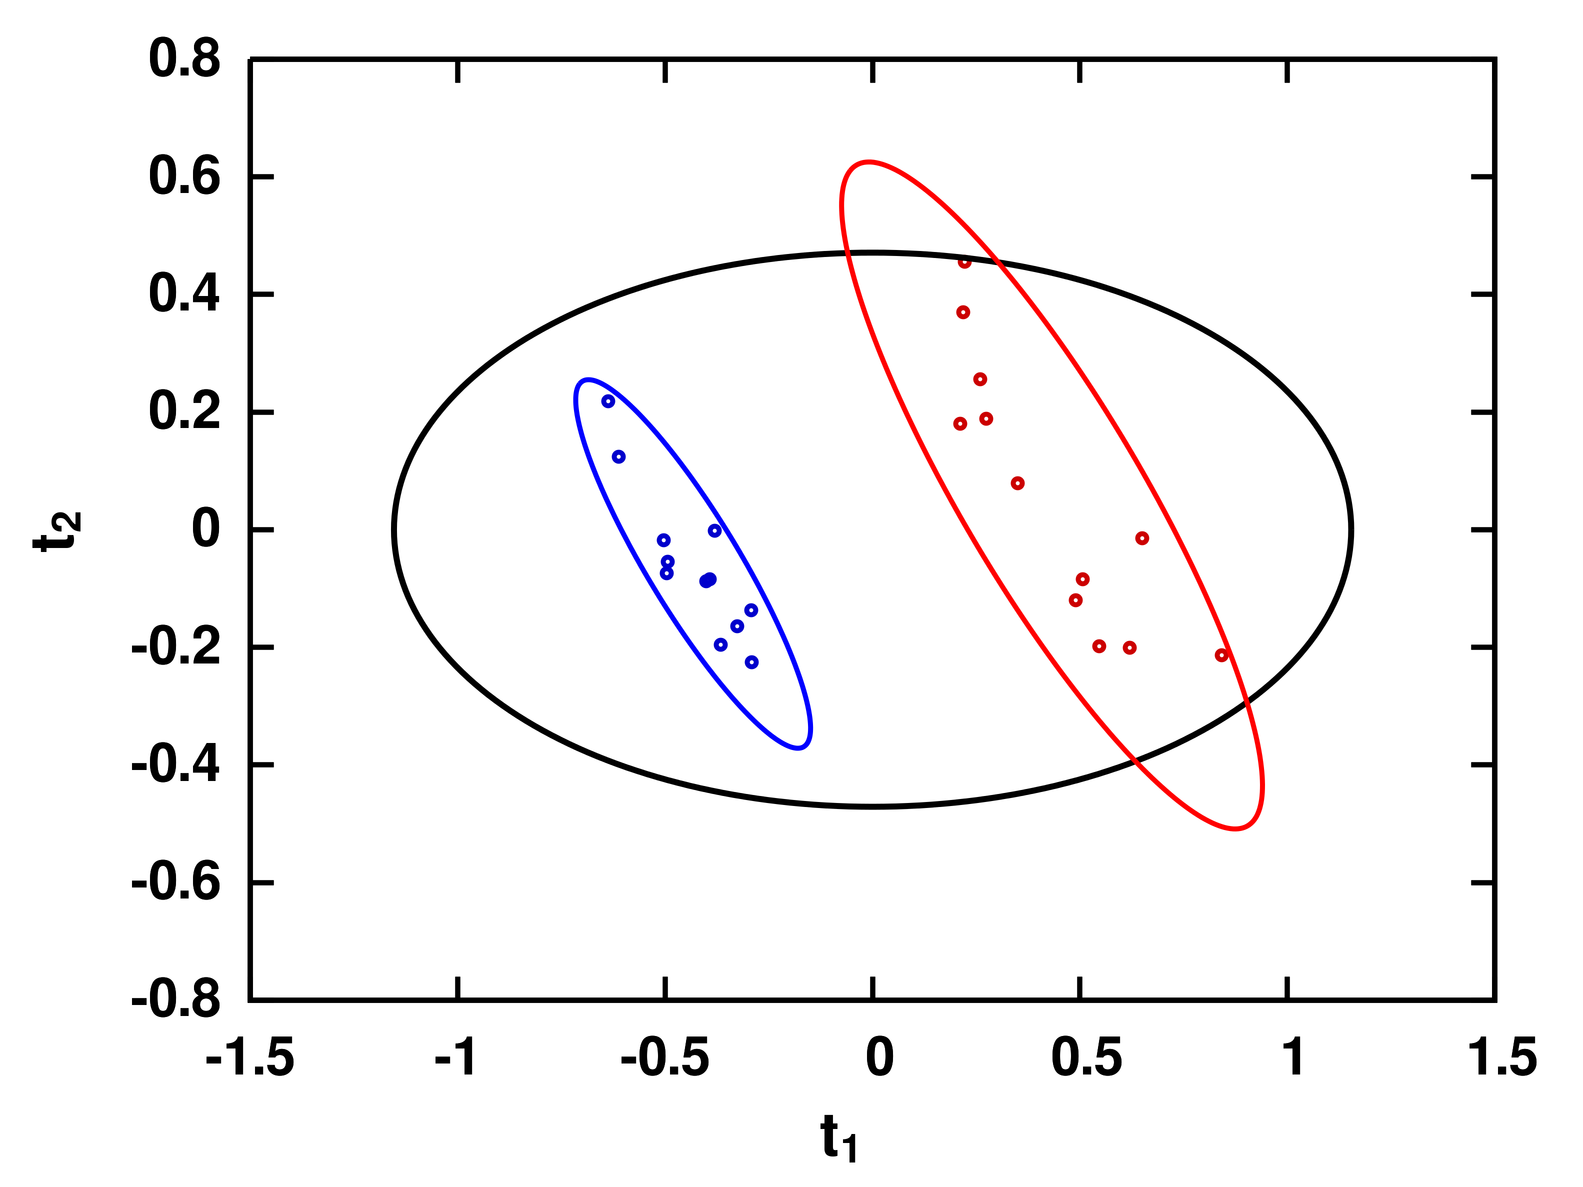
\includegraphics[width=3.25in]{figs/gaibin/04-scores.png}
\caption
      [PCA Scores of a GAI-binned Tensor.]{
  {\bf PCA Scores of a GAI-binned Tensor.}
  \\
  Principal component analysis scores resulting from modeling the GAI-binned
  \hcnmr{} HSQC liver data matrix, indicating a high degree of separation
  between experimental groups. Model \rsqx{} and \qsq{} were 0.68 and 0.64 for
  the first principal component ($t_1$) and 0.12 and 0.09 for the second
  ($t_2$). Class separations of this magnitude are readily achievable using
  data matrices generated by GAI-binning, due in large part to the low variable
  counts it generally produces.
}
\label{figure.8.4}
\end{SCfigure}

\begin{doublespace}
Backscaled predictive OPLS-DA loadings of the vectorized \hcnmr{} HSQC spectral
data tensors (\figref{8.5}{Figure 8.5}) lend further support for the use of
multidimensional binning in metabolic fingerprinting studies. Even when
vectorization is performed in place of integration to produce a data matrix,
binning offers an effective means of variable selection: only 10,474 of 65,858
variables (16\%) were retained when GAI-binning was used as a pre-filter prior
to modeling the liver data. A similar reduction was observed in the fibroblast
dataset, where GAI-binning retained 18,789 of 184,212 total variables for
a 90\% reduction in dimensionality. These substantially reduced variable
counts offered by binning translate to more well-conditioned bilinear
modeling problems. As the dimensionality of the input dataset is
increased further, the reductions in variable count afforded by
multidimensional binning are expected to become even
more dramatic. While the variable counts produced by vectorization of uniformly
binned data tensors are comparable to those from GAI-binning, it is critical to
recognize that the uniformly binned regions contain more noise data points than
their GAI-binned counterparts, and thus offer a less efficient dimensionality
reduction.
\\\\
Spectral regions produced by GAI-binning (\figref{8.2}{Figure 8.2})
demonstrate several important properties of the combined binning and noise
removal processes. Because $t_1$ noise and truncation artifacts yield
phase-incoherent negative spectral excursions after Fourier
transformation, ``unrelaxed'' GAI-binning ($R = 1$) tends to
preferentially subdivide near such regions, producing
elongated bins along the $F_1$ dimension. Decreasing the resolution parameter
from its maximum value shrinks these bins to contain only true signals. Thus,
an objective rule for determining an optimal resolution parameter during
binning is to decrease $R$ until all bins shrink to contain a minimal amount
of noise. Once an optimal resolution parameter has been identified, a suitable
noise threshold ($k$) must be determined such that all noise bins are removed
without loss of bins containing weak signals. However, once $R$ and $k$ have
been determined for a given set of experimental conditions, they may be applied
during GAI-binning to any data collected at later times under the same
conditions to achieve ideal results. The selections of resolution parameter
($R = 0.1$) and noise threshold ($k = 3$) made in this work were identified
according to the above criteria through a manual visual examination of the
binning results, but it is conceivable that objective metrics of these criteria
could be constructed that facilitate automated determination of these
parameters.
\\\\
Finally, like AI-binning, the execution time of GAI-binning scales
quadratically with the number of spectral data points, and scales approximately
linearly with both the number of spectral dimensions and the number of
observations. Typical runtimes for binning two-dimensional datasets range from
seconds to a few minutes, depending mostly on the data point count. Thus,
while zero-filling may be used to increase the digital resolution of data
being input into GAI-binning, it should be applied sparingly to avoid
unnecessarily long computation times during bin region determination.
\end{doublespace}

\begin{figure}[hb!]
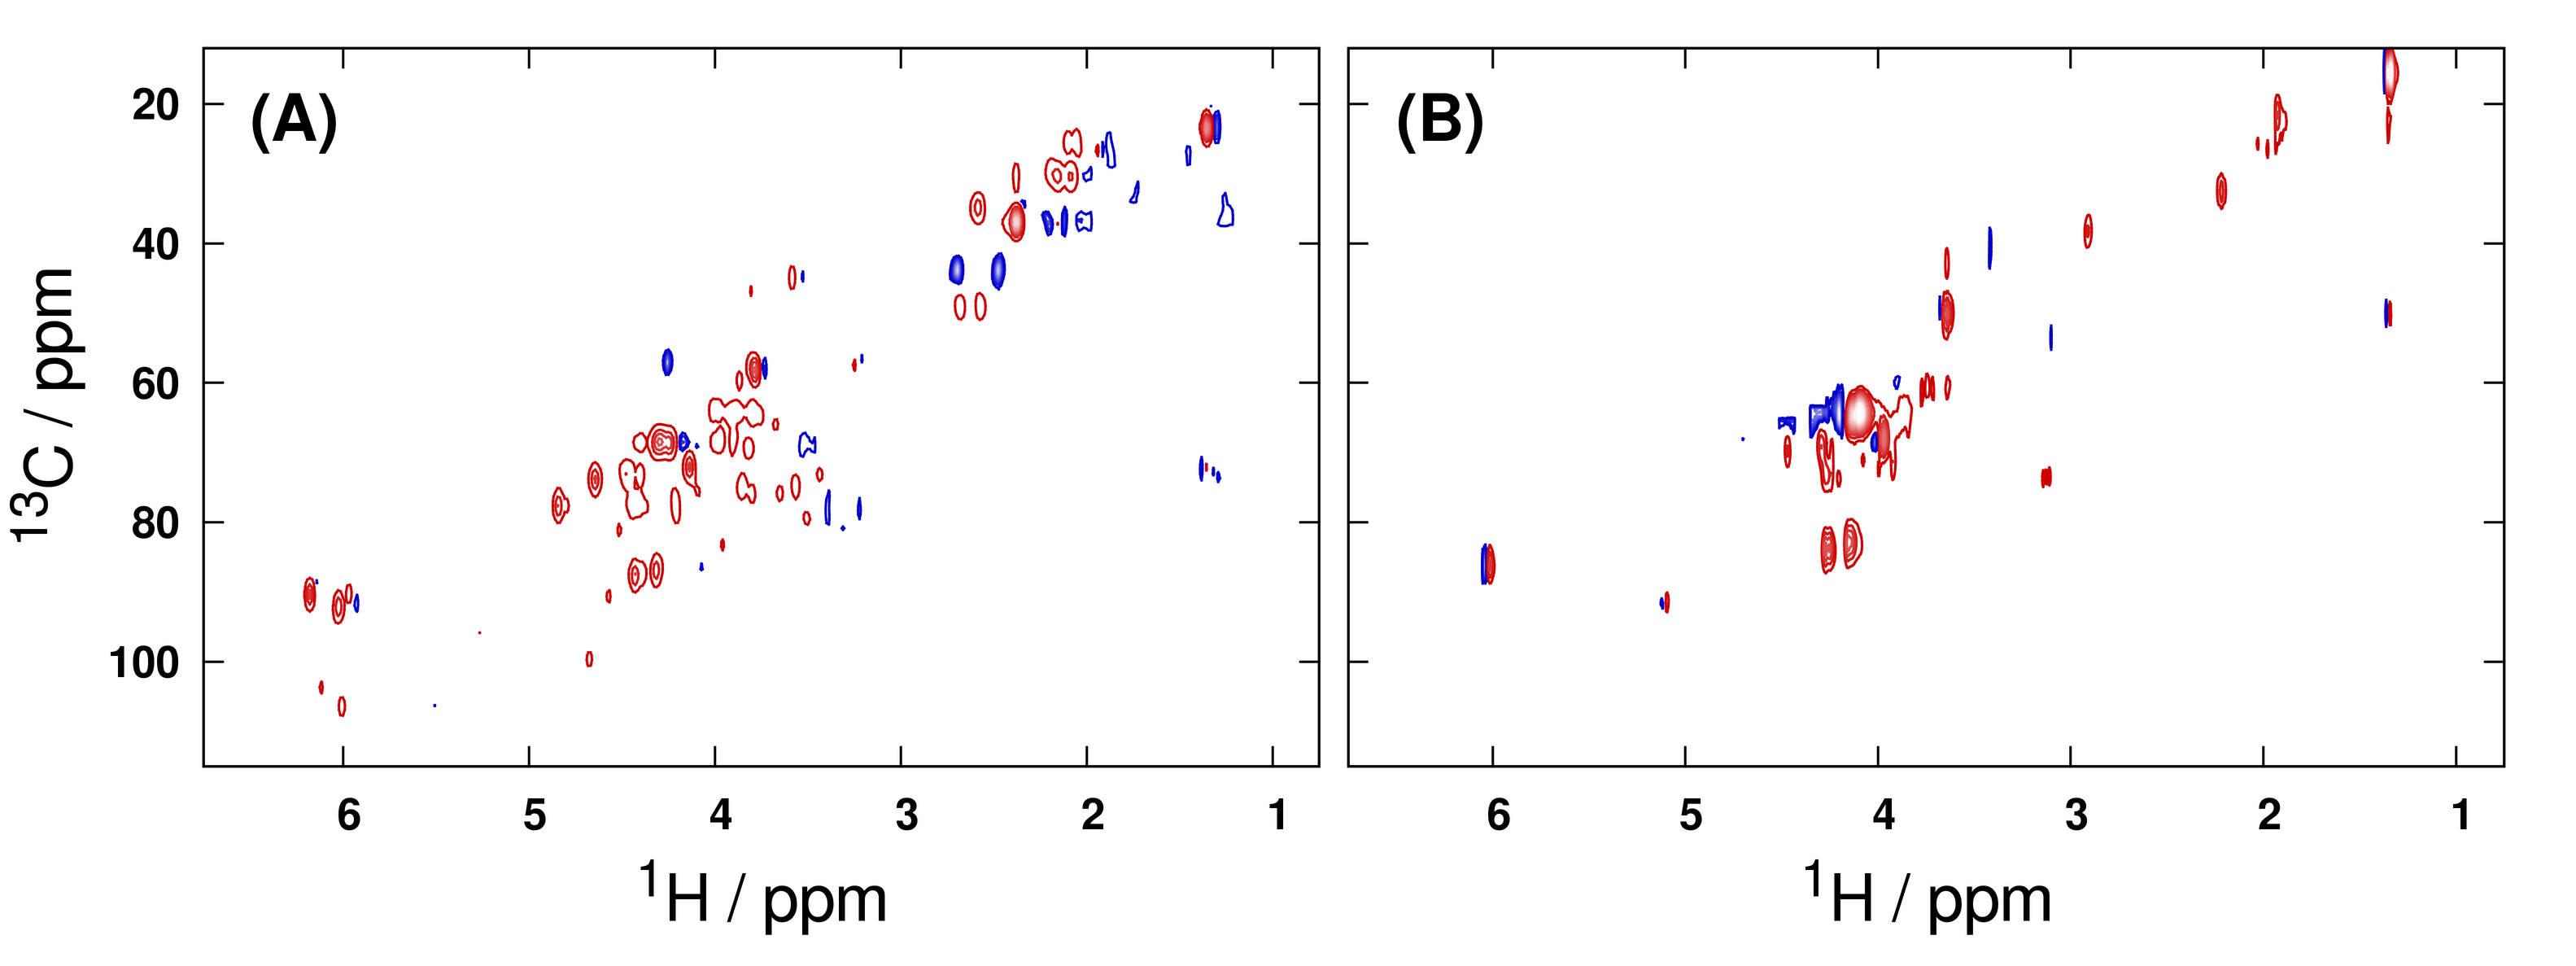
\includegraphics[width=6in]{figs/gaibin/05-loadings.png}
\caption
      [Pseudospectral HSQC Loadings.]{
  {\bf Pseudospectral HSQC Loadings.}
  \\
  Backscaled full-resolution pseudospectral loadings from OPLS-DA modeling of
  the GAI-reduced ({\bf A}) liver and ({\bf B}) fibroblast \hcnmr{} HSQC data
  tensors. Positive and negative loadings are represented by red and blue
  contours, respectively.
}
\label{figure.8.5}
\end{figure}

\section{Conclusions}

\begin{doublespace}
Generalized Adaptive Intelligent binning is a logical extension of the
previously described Adaptive Intelligent binning algorithm
\cite{demeyer:anchem2008} to multidimensional datasets, and provides a
model-free alternative to peak-fitting and peak-picking as a means of variable
selection in multivariate analyses. Furthermore, GAI-binning is a more
intelligent method to extract signal regions from multidimensional spectral
data tensors than uniform binning, and may be used to generate very
low-dimensionality data matrices via multiple integration or efficiently
noise-filtered data matrices via vectorization. The C++ implementations of
1D and 2D GAI-binning used in this work are freely available as part of the
MVAPACK software package \cite{worley:acscb2014} introduced in
\hyperlink{chapter.5}{Chapter 5}.
\end{doublespace}

\newpage
\section{Permutation Test Results}

\begin{figure}[ht!]
\includegraphics[width=6in]{figs/gaibin/06-perm-unif-int.png}
\caption
      [Response Permutation Test: Uniform integration.]{
  {\bf Response Permutation Test: Uniform integration.}
  \\
  Response permutation test results for OPLS-DA models from the uniformly
  binned (integrated) liver ({\bf A}, {\bf B}) and fibroblast
  ({\bf C}, {\bf D}) data tensors. Model fit (\rsqy{}) statistics
  ({\bf A}, {\bf C}) are shown in blue, and model predictive ability (\qsq{})
  statistics ({\bf B}, {\bf D}) are shown in green. True values of \rsqy{} and
  \qsq{} are represented by vertical bars, and null distributions are computed
  through kernel density estimation of the values from permutation. Scatter
  plots of the permutation (null) \rsqy{} and \qsq{} statistics are shown in
  the lower panes.
}
\label{figure.8.6}
\end{figure}

\begin{figure}[ht!]
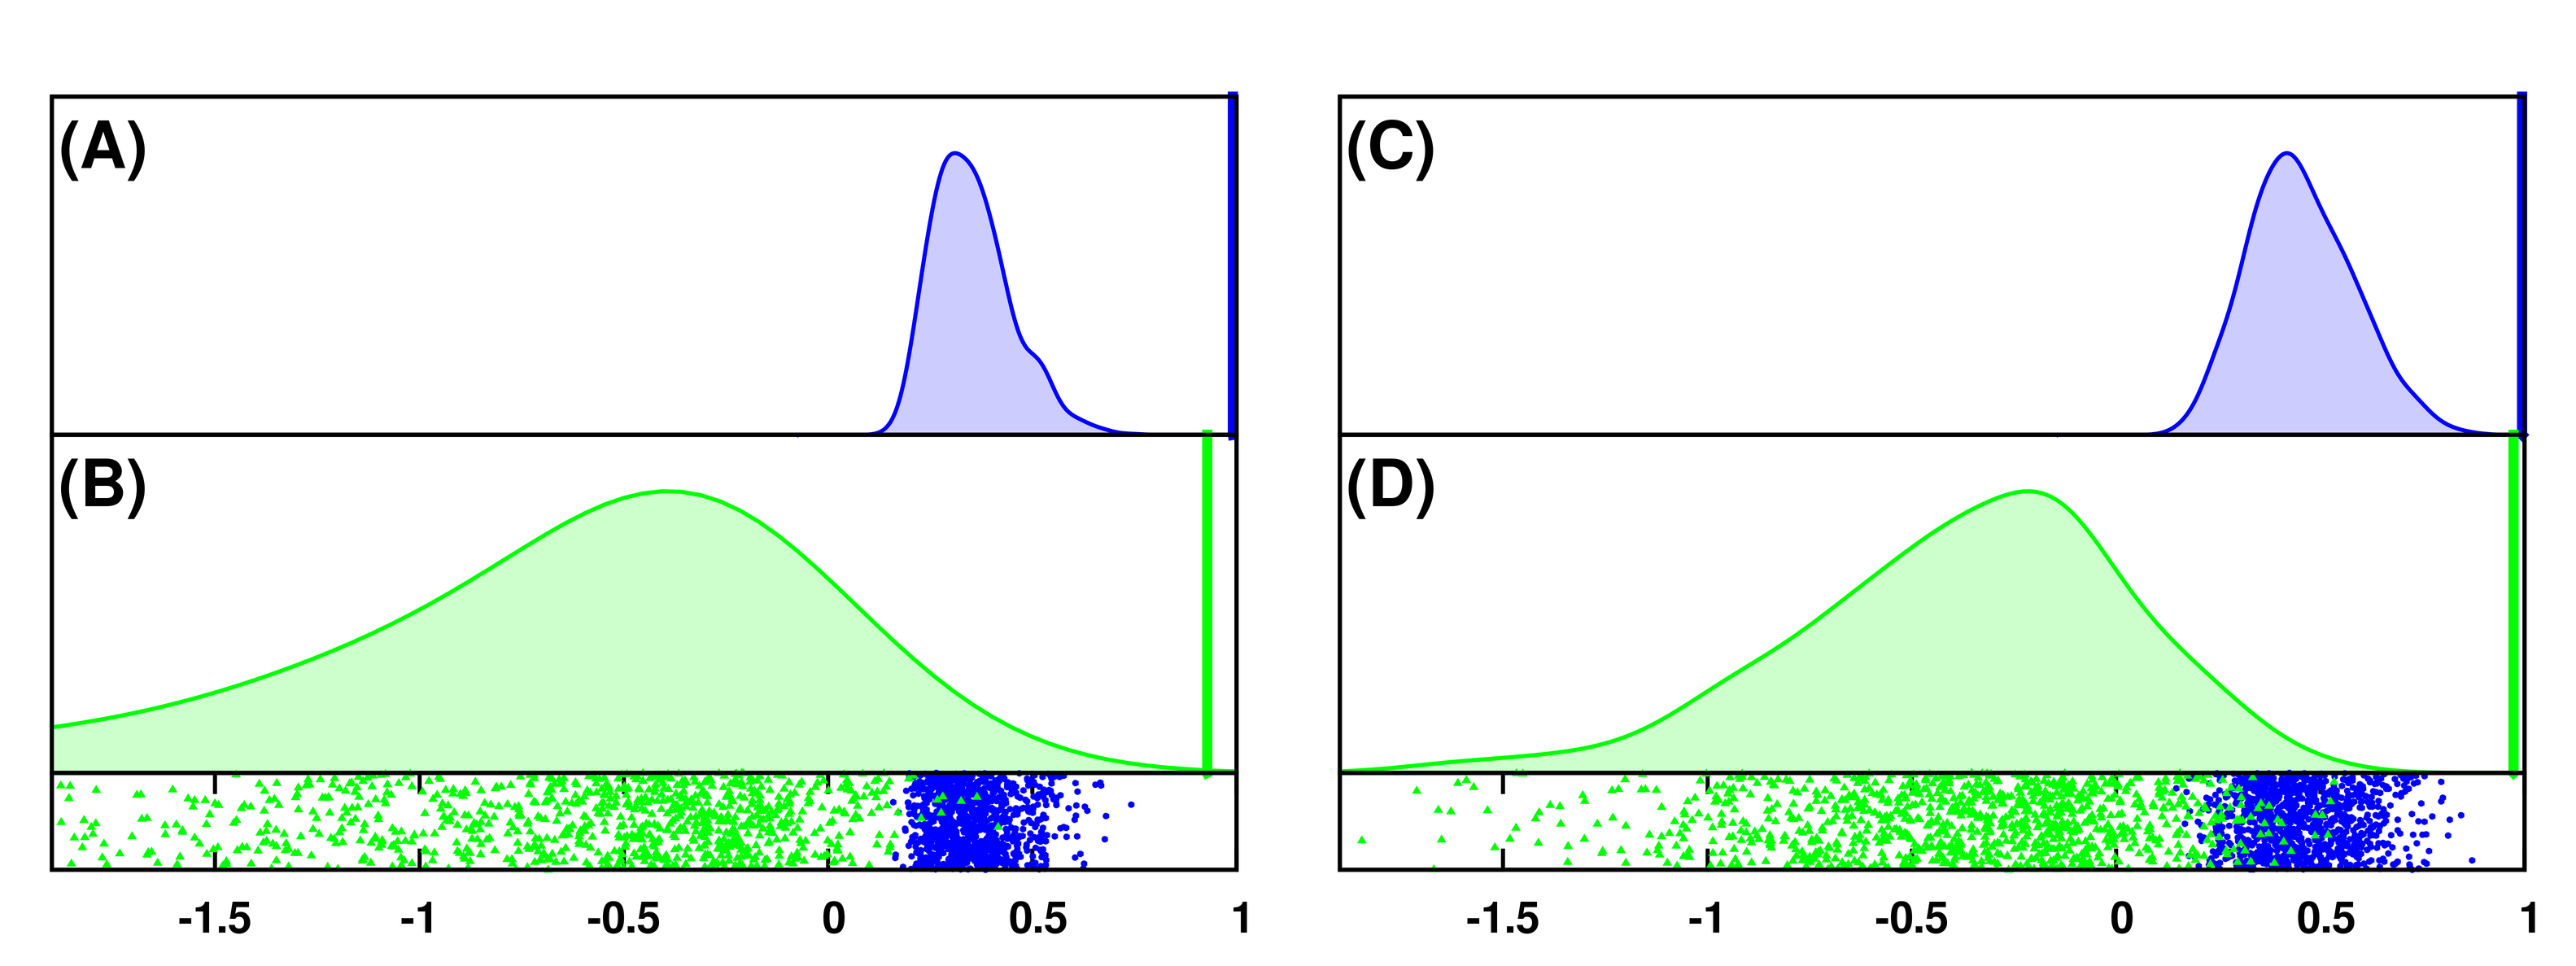
\includegraphics[width=6in]{figs/gaibin/07-perm-gai-int.png}
\caption
      [Response Permutation Test: GAI-integration.]{
  {\bf Response Permutation Test: GAI-integration.}
  \\
  Response permutation test results for OPLS-DA models from the GAI-binned
  (integrated) liver ({\bf A}, {\bf B}) and fibroblast
  ({\bf C}, {\bf D}) data tensors. See the caption of Figure 8.6 for a
  complete description of the figure contents.
}
\label{figure.8.7}
\end{figure}

\begin{figure}[ht!]
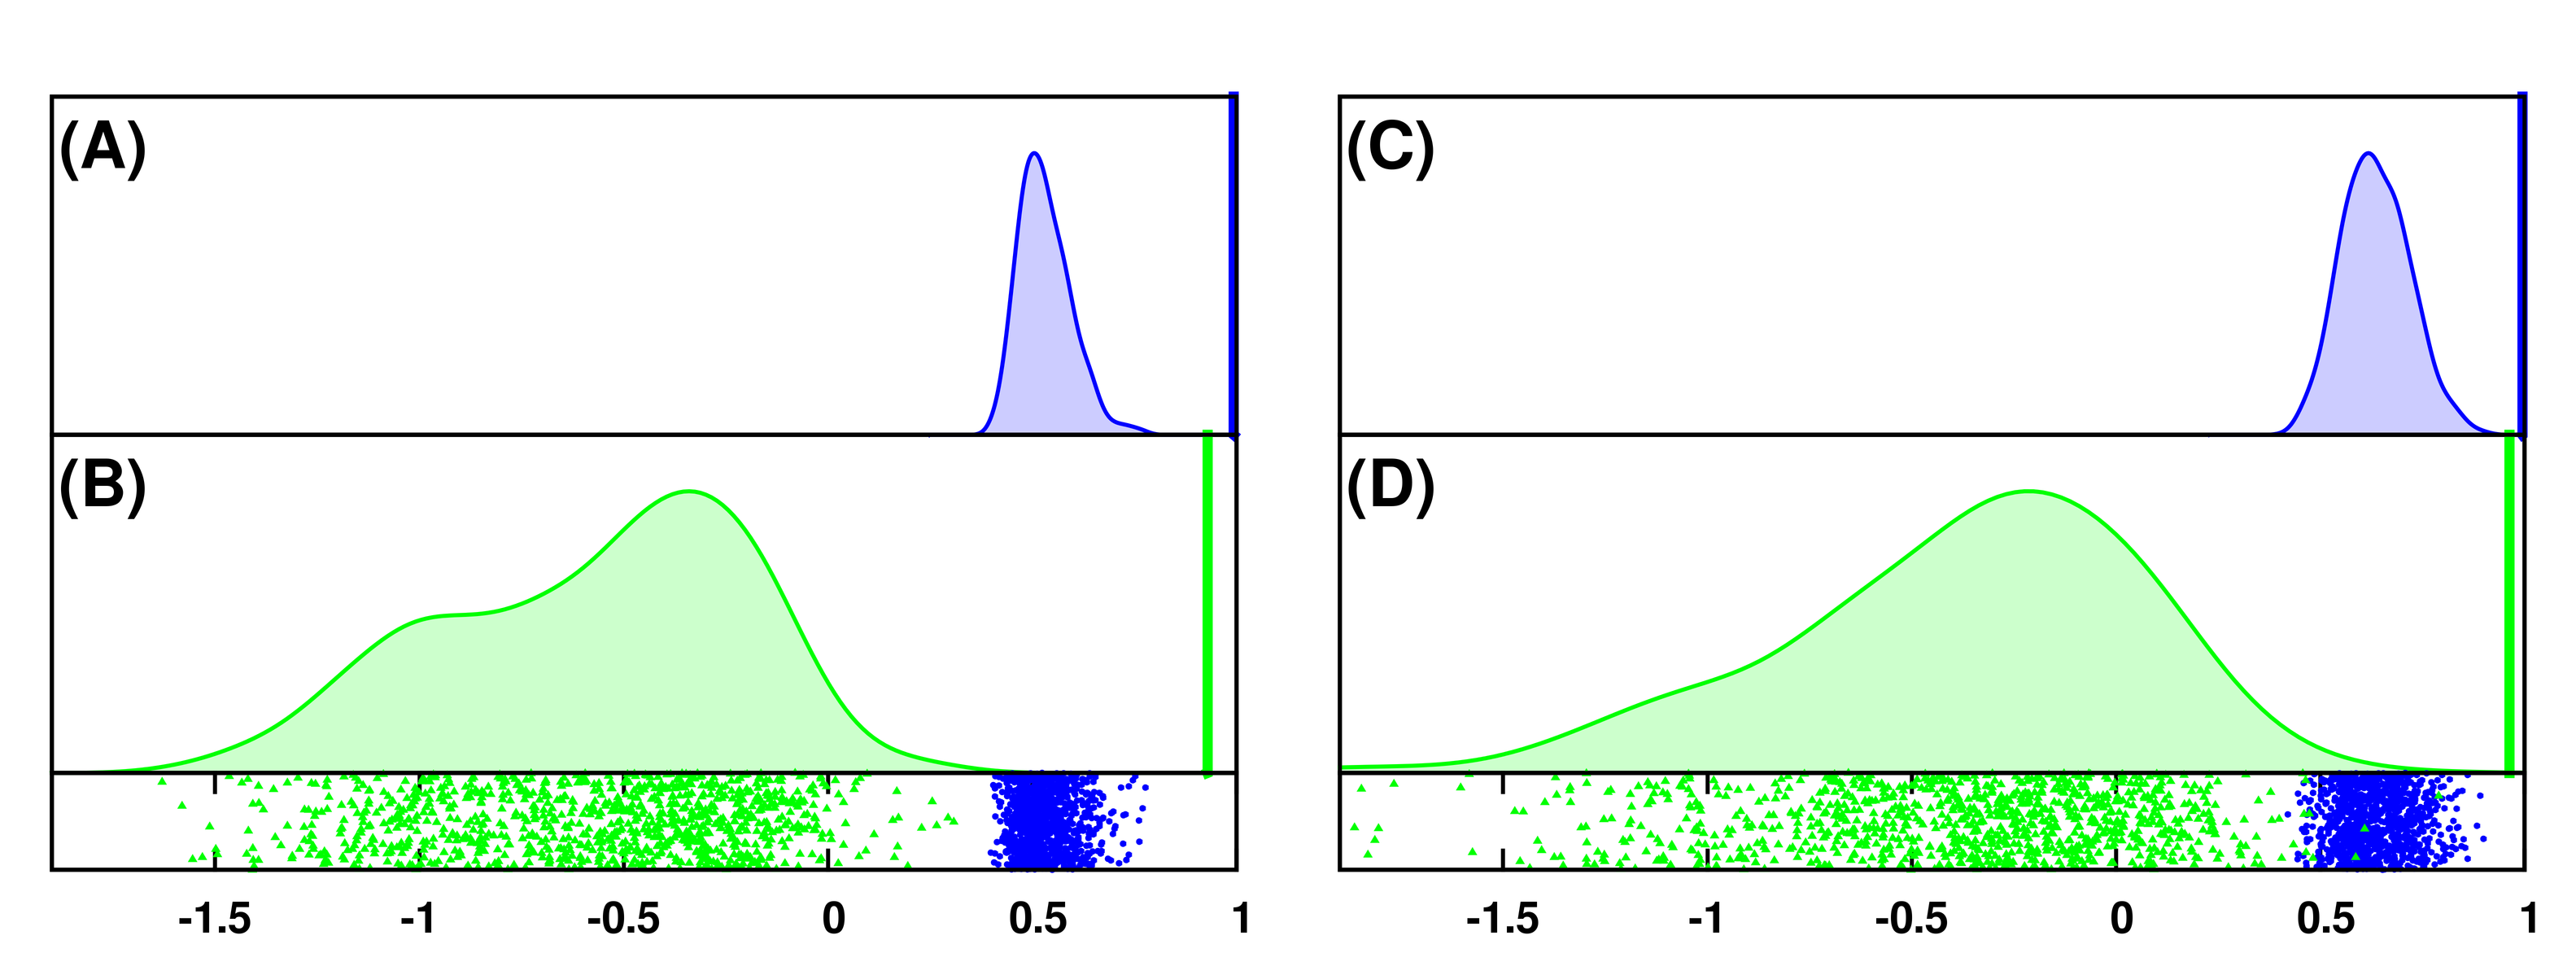
\includegraphics[width=6in]{figs/gaibin/08-perm-unif-vec.png}
\caption
      [Response Permutation Test: Uniform vectorization.]{
  {\bf Response Permutation Test: Uniform vectorization.}
  \\
  Response permutation test results for OPLS-DA models from the uniformly
  binned (vectorized) liver ({\bf A}, {\bf B}) and fibroblast
  ({\bf C}, {\bf D}) data tensors. See the caption of Figure 8.6 for a
  complete description of the figure contents.
}
\label{figure.8.8}
\end{figure}

\begin{figure}[ht!]
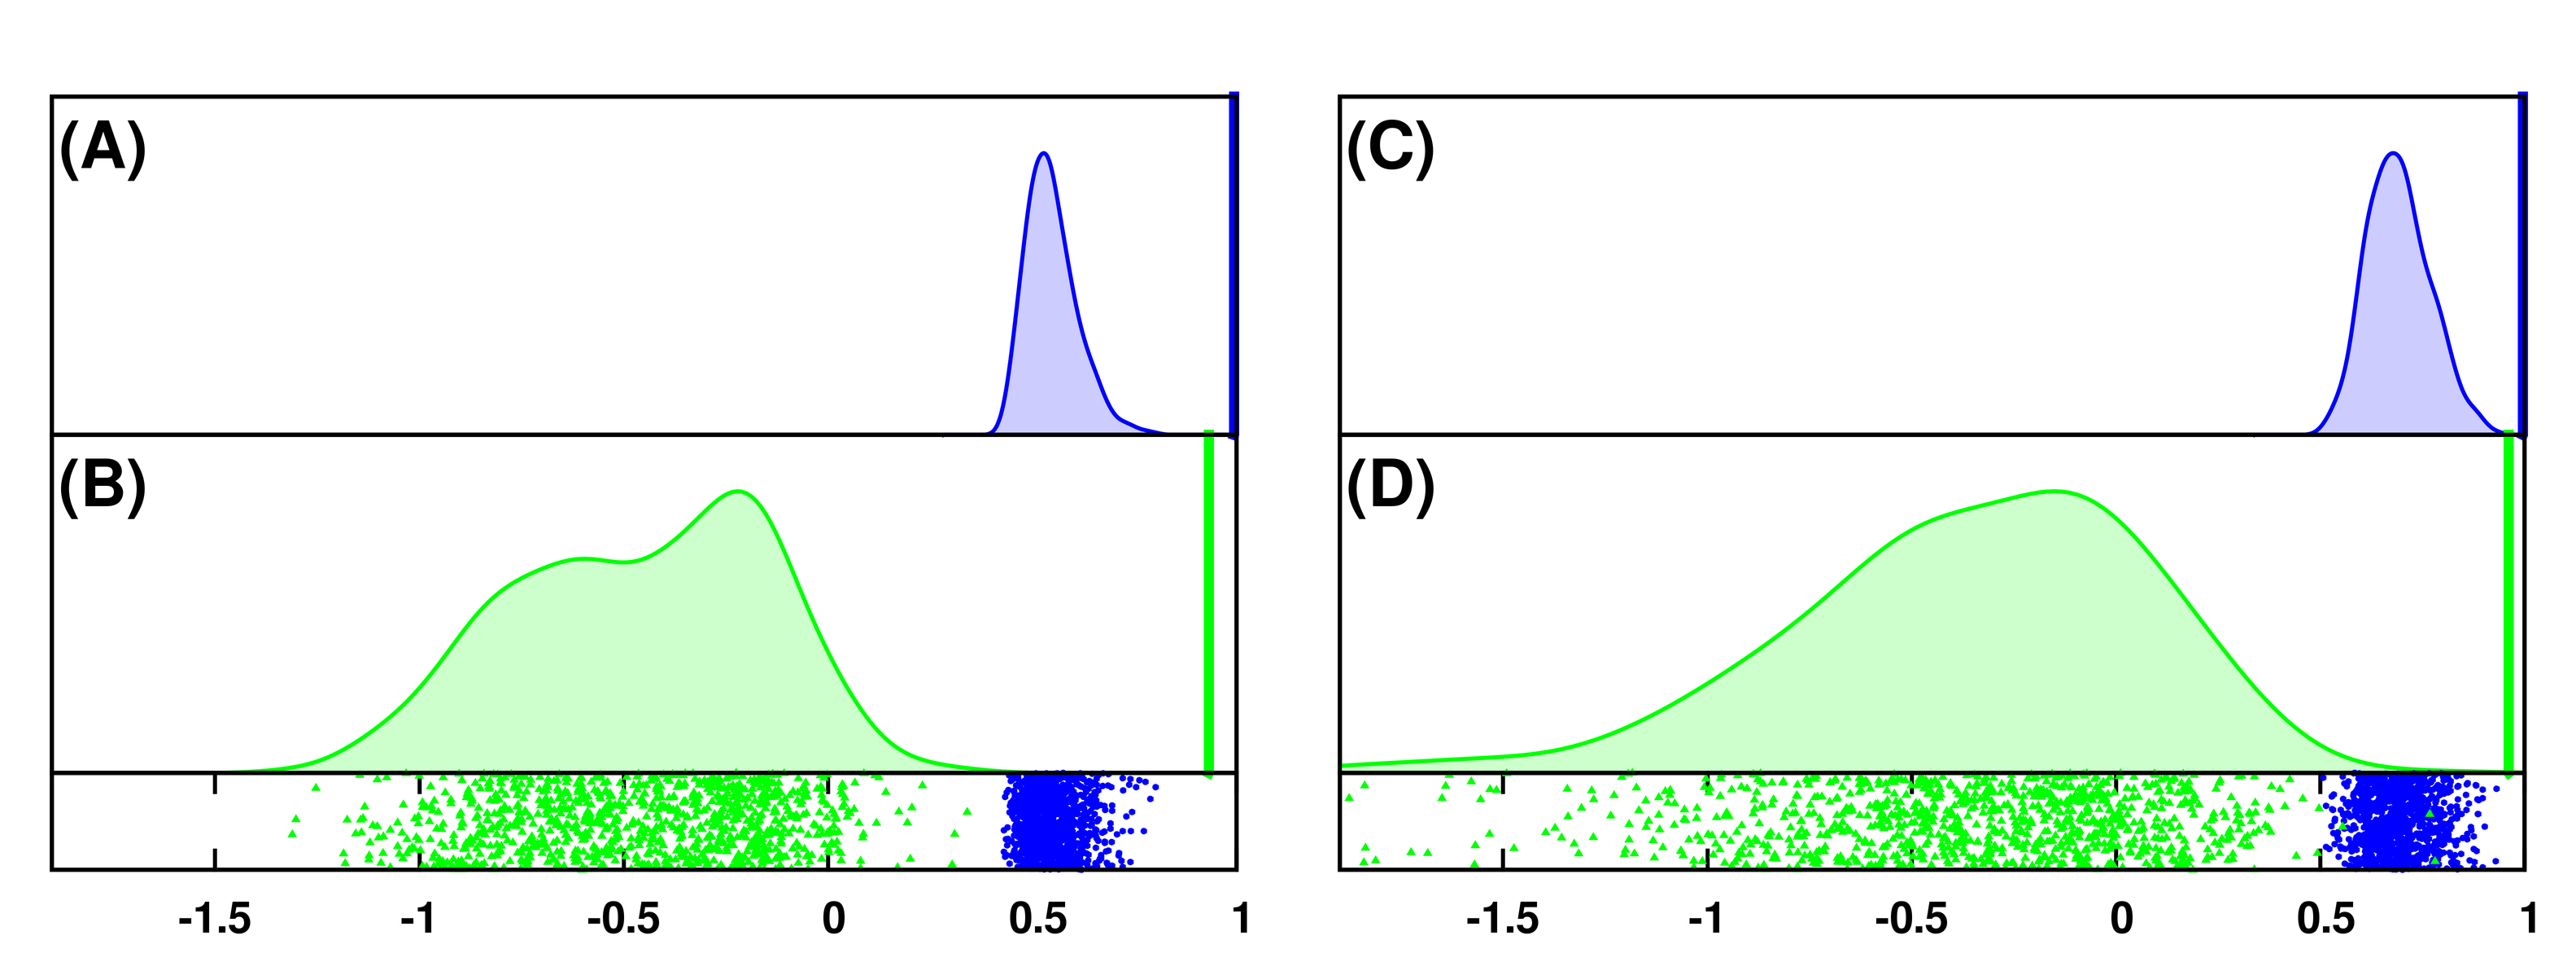
\includegraphics[width=6in]{figs/gaibin/09-perm-gai-vec.png}
\caption
      [Response Permutation Test: GAI-vectorization.]{
  {\bf Response Permutation Test: GAI-vectorization.}
  \\
  Response permutation test results for OPLS-DA models from the GAI-binned
  (vectorized) liver ({\bf A}, {\bf B}) and fibroblast
  ({\bf C}, {\bf D}) data tensors. See the caption of Figure 8.6 for a
  complete description of the figure contents.
}
\label{figure.8.9}
\end{figure}

\newpage
\bibliographystyle{abbrv}
\bibliography{bworley}

